\documentclass[conference]{IEEEtran}
\ifCLASSINFOpdf
  \usepackage[pdftex]{graphicx}
  % declare the path(s) where your graphic files are
  % \graphicspath{{../pdf/}{../jpeg/}}
  % and their extensions so you won't have to specify these with
  % every instance of \includegraphics
  % \DeclareGraphicsExtensions{.pdf,.jpeg,.png}
\else
  % or other class option (dvipsone, dvipdf, if not using dvips). graphicx
  % will default to the driver specified in the system graphics.cfg if no
  % driver is specified.
  \usepackage[dvips]{graphicx}
  % declare the path(s) where your graphic files are
  % \graphicspath{{../eps/}}
  % and their extensions so you won't have to specify these with
  % every instance of \includegraphics
  % \DeclareGraphicsExtensions{.eps}
\fi

\usepackage{listings}
\usepackage{color}
\usepackage{xcolor}
\usepackage{cite}

\usepackage[cmex10]{amsmath}
%\usepackage[norelsize]{algorithm2e}
%\usepackage{algorithmic}
%\usepackage{array}
%\usepackage{mdwmath}
%\usepackage{mdwtab}
%\usepackage{eqparbox}
%\usepackage[tight,footnotesize]{subfigure}
%\usepackage[caption=false]{caption}
%\usepackage[font=footnotesize]{subfig}
%\usepackage[caption=false,font=footnotesize]{subfig}
%\usepackage{fixltx2e}
%\usepackage{stfloats}
\usepackage{url}
\usepackage{booktabs}
\usepackage{todonotes}
\hyphenation{guided-io}


\begin{document}

\title{POSTER: Optimizing Scientific File I/O Patterns using Advice Based Knowledge}

\author{
%\IEEEauthorblockN{Giuseppe Congiu}
%\IEEEauthorblockA{Emerging Technology Group\\
%Xyratex Technology LTD\\
%Havant, United Kingdom\\
%Email: giuseppe\underline{ }congiu@xyratex.com}
%\and
%\IEEEauthorblockN{Matthias Grawinkel,\\Federico Padua} %Tim S\"u\ss{}, Andr\'e Brinkmann}
%\IEEEauthorblockA{Zentrum f\"ur Datenverarbeitung\\
%Johannes Gutenberg-University Mainz, Germany\\
%Email: \{meatz,padua\}@uni-mainz.de}
%\and
%\IEEEauthorblockN{James Morse}
%\IEEEauthorblockA{Emerging Technology Group\\
%Xyratex Technology LTD\\
%Havant, United Kingdom\\
%Email: james\underline{ }morse@xyratex.com}
%\and
%\IEEEauthorblockN{Tim S\"u\ss{}, Andr\'e Brinkmann}
%\IEEEauthorblockA{Zentrum f\"ur Datenverarbeitung\\
%Johannes Gutenberg-University Mainz, Germany\\
%Email: \{t.suess,brinkman\}@uni-mainz.de}}

\IEEEauthorblockN{Giuseppe Congiu\IEEEauthorrefmark{1}, Matthias Grawinkel\IEEEauthorrefmark{2}, Federico Padua\IEEEauthorrefmark{2}, James Morse\IEEEauthorrefmark{1}, Tim S\"u\ss{}\IEEEauthorrefmark{2}, Andr\'e Brinkmann\IEEEauthorrefmark{2}}
\IEEEauthorblockA{\IEEEauthorrefmark{1}Emerging Technology Group Seagate Technology Havant, United Kingdom\\
Email: \{giuseppe\underline{ }congiu, james\underline{ }morse\}@xyratex.com}
\IEEEauthorblockA{\IEEEauthorrefmark{2}Zentrum f\"ur Datenverarbeitung Johannes Gutenberg-University Mainz, Germany\\
Email: \{grawinkel, padua, t.suess, brinkman\}@uni-mainz.de}}
\maketitle

% What is the abstract word limit for this conference?
%\begin{abstract}
%The performance gap between processing and I/O represents a serious scalability limitation for scientific applications running on high-end computing clusters. Parallel file systems often provide mechanisms that allow programmers to disclose their I/O pattern knowledge to the lower layers of the I/O stack through a hints API. This information can be used by the file system to boost the application performance, for example, through data prefetching. Unfortunately, programmers rarely make use of these features, missing the opportunity to exploit the full potential of the storage system. Additionally, scientific applications frequently perform small non-contiguous accesses to files using the POSIX I/O interface. This makes it impossible for them to take advantage of automatic optimizations, such as collective I/O or data-sieving enabled by the MPI I/O middleware. As a result these applications perform poorly. More significantly they can negatively impact the whole storage system's efficiency. \\
%In this paper we propose an advice infrastructure to optimize file I/O patterns in scientific applications, allowing users and administrators to directly control the I/O behavior of their applications without modifying them. This is done by exploiting the hints API provided by the back-end file system to guide data prefetching. %The required prefetching information is annotated in a configuration file using a generic syntax and afterwards transparently translated into the corresponding file system subroutine calls. 
%We demonstrate that our approach is effective in converting numerous small read requests into a few larger requests and that by doing so, it increases the I/O bandwidth, reduces the number of I/O requests reaching the back-end storage devices and ultimately the application running time. Moreover, we also propose a Linux Kernel modification that allows network file systems, specifically lustre, to work with our advice infrastructure through the posix\_fadvise interface.
%\end{abstract}

\section{Introduction}
\label{sec: intro}
The performance gap between processing and I/O represents a serious scalability limitation for scientific applications running on high-end computing clusters. Parallel file systems often provide mechanisms that allow programmers to disclose their I/O pattern knowledge to the lower layers of the I/O stack through a hints API. This information can be used by the file system to boost the application performance, for example, through data prefetching. Unfortunately, programmers rarely make use of these features, missing the opportunity to exploit the full potential of the storage system. Additionally, scientific applications frequently perform small non-contiguous accesses to files using the POSIX I/O interface. This makes it impossible for them to take advantage of automatic optimizations, such as collective I/O or data-sieving enabled by the MPI I/O middleware. As a result these applications perform poorly. More significantly they can negatively impact the whole storage system's efficiency.
%In this paper we propose an advice infrastructure to optimize file I/O patterns in scientific applications, allowing users and administrators to directly control the I/O behavior of their applications without modifying them. This is done by exploiting the hints API provided by the back-end file system to guide data prefetching. The required prefetching information is annotated in a configuration file using a generic syntax and afterwards transparently translated into the corresponding file system subroutine calls. 
%We demonstrate that our approach is effective in converting numerous small read requests into a few larger requests and that by doing so, it increases the I/O bandwidth, reduces the number of I/O requests reaching the back-end storage devices and ultimately the application running time. Moreover, we also propose a Linux Kernel modification that allows network file systems, specifically lustre, to work with our advice infrastructure through the posix\_fadvise interface.

%The gap between hard disk drives (HDDs) performance and processors computing power, better known as I/O performance gap problem, represents a serious scalability limitation especially for scientific applications running on High End Computing (HEC) clusters. 
%Parallel File Systems (PFSs) such as Lustre~\cite{Braam02}, PVFS~\cite{CarnsLRT} and GPFS~\cite{SchmuckH02}, just to mention a few, try to bridge this gap by striping files across multiple storage devices and providing multiple parallel data paths to increase the aggregate I/O bandwidth and the number of IOPS. The ROMIO middleware\footnote{Implementation of MPI I/O specifications from Argone National Laboratory included in MPICH package (http://www.mpich.org/).} extends the POSIX I/O interface typically provided by PFSs with a richer parallel I/O interface, and through the Abstract Device I/O (ADIO) driver~\cite{ThakurGL96} enables transparent file access optimizations based on two-phase I/O and data sieving to adapt I/O patterns to the characteristics of the underlying file system~\cite{ThakurGL99}~\cite{Ying08}~\cite{ProstTHKW00}.

%Nevertheless, as Carns et al. have pointed out in their study~\cite{CarnsHABLLR11} most of the scientific applications running on big clusters today still use the POSIX I/O interface to access their data. Furthermore, it has also been ascertained that using POSIX I/O to access non-contiguous regions of files causes extremely poor performance in the case of PFSs~\cite{ChingCLP06}. Indeed, PFSs provide best I/O bandwidth performance for large contiguous requests while they typically provide only a fraction of the maximum bandwidth in the opposite case. This is primarily due to the high number of remote procedure calls generated by the file system clients that overwhelms I/O servers and the resulting high number of HDDs' head movements in every I/O server (seek overhead). 

%Currently there is no available solution to overcome limitations caused by non-optimal file I/O patterns generated by applications, except to re-write them. In this context, the Linux kernel provides users with the capability to communicate access pattern information to the local file system through the \texttt{posix\_fadvise()}~\cite{AdviseAPI} system call. The file system can use this information to improve page cache efficiency, for example, by prefetching (or releasing) data that will (or will not) be required soon in the future or by disabling read-ahead in the case of random read patterns. However, \texttt{posix\_fadvise()} is barely used in practice and has intrinsic limitations that discourage its employment in real applications. 
%TODO: is there a citation for this 'barely' claim?

%The two most used PFSs in HEC clusters nowadays, IBM GPFS and Lustre, are both POSIX compliant. Nevertheless, neither of them support the POSIX advice mechanism previously described. GPFS compensates for the lack of POSIX advice support through a hints API that users can access by linking their programs against a service library. Hints are passed to GPFS through the \texttt{gpfs\_fcntl()}~\cite{GPFSHINTS} function and can be used to guide prefetching (or releasing) of file blocks in the page pool\footnote{GPFS pinned memory used for file system caching.}. However, unlike POSIX advice, GPFS hints are not mandatory and can be discarded by the file system if certain requirements are not met. Lustre, on the other hand, does not provide any client side mechanism similar to GPFS hints or POSIX advice. Recently a new Lustre advice mechanism has been proposed by DDN during the Lustre User Group 2014 (LUG14) in Miami~\cite{Comer14}. The difference in the DDN approach is that it provides control over the storage servers (OSSs) cache instead of the file system client cache.
%TODO: why is your approach better? Yours has the penalty of moving the data over the wire into the client cache. Perhaps the approaches are complimentary, you address "I will want this data", they address "someone will want this data, but _they_ may not know it yet"

In this paper we propose and evaluate a novel advice infrastructure able to optimize file access patterns at run-time through data prefetching using these hints mechanisms (Figure~\ref{figure: softwarestack}). 
\begin{figure}[!htb]
  \centering
  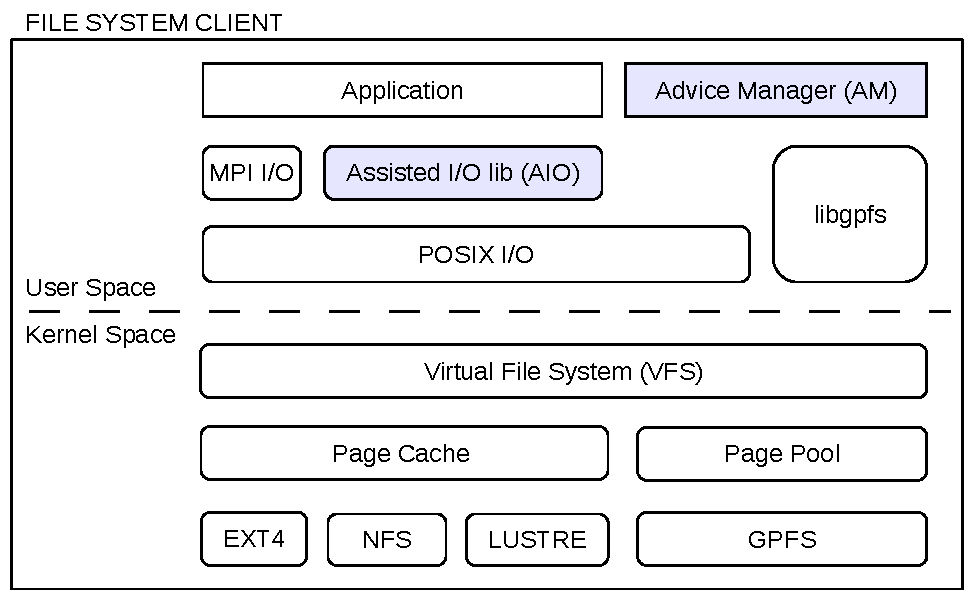
\includegraphics[width=0.35\textwidth]{../figures/softwarestack}
  \caption{I/O software stack of the advice infrastructure. \textit{Interposing I/O Library} and \textit{Advice Manager} communicate through UNIX domain sockets. %The AM binds its socket to the local file system pathname \texttt{/tmp/channel}, while the IL connects its socket to the same pathname; exactly in the same way they would bind and connect to an IP address if they were located on different nodes in the network. Unix domain sockets are used to pass ancillary data as well as custom messages between the two software entities. 
  %Data can reside in a local Linux file system, in Lustre or in GPFS.
  }
  \label{figure: softwarestack}
\end{figure}
Our advice infrastructure communicates file I/O pattern information to the file system on behalf of running applications using a dedicated process that we call \textit{Advice Manager}. Processes access their files using an \textit{Interposing I/O Library} that transparently forwards intercepted requests to the local \textit{Advice Manager}. This uses \texttt{posix\_fadvise()} and \texttt{gpfs\_fcntl()} to prefetch (or release) data into (or from) the client's file system data cache. The \textit{Interposing I/O Library} controls for which files advice or hints should be given, while the \textit{Advice Manager} controls how much data to prefetch (or release) from each file. Monitored file paths and prefetching information are contained in a configuration file that can be generated either manually or automatically once the I/O behaviour of the target application is known. The configuration file mechanism allows us to decouple the specific hints API provided by the back-end file system from the generic interface exposed to the final user thus making our infrastructure portable.

With this approach we are able to generate POSIX advice and GPFS hints for applications that do not use them but can receive a benefit from their use. We accomplish this asynchronously, with very low overhead, and without any modification of the original application. We demonstrate that our approach is effective in improving the I/O bandwidth, reducing the number of I/O requests and reducing the execution time of a `ROOT'\footnote{Data analysis framework developed at CERN (http://root.cern.ch/drupal).} based application.

Additionally, we propose and evaluate a modification to the Linux kernel that makes it possible for Lustre and other networked file systems to participate in activity triggered by the \texttt{posix\_fadvise()} system call, thus allowing it to take advantage of our advice infrastructure benefits.
%\begin{figure}[!htb]
%  \centering
%  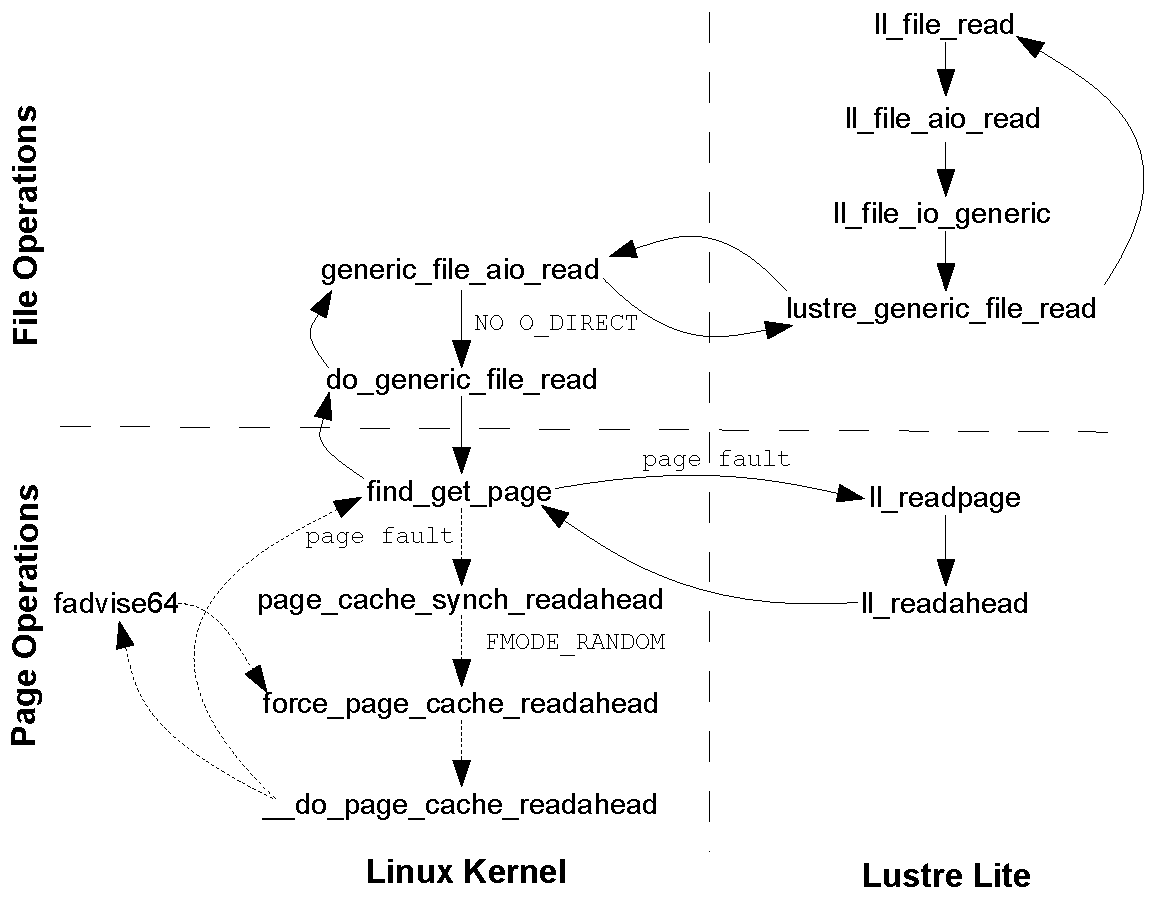
\includegraphics[width=0.4\textwidth]{../figures/kernel}
%  \caption{Simplified function call graph for the read operation in Lustre. %For page operations in the Linux kernel 
%  The picture also shows the call graph for local reads and \texttt{POSIX\_FADV\_WILLNEED} in the \texttt{posix\_fadvise()} implementation (dashed line).}
%  \label{figure: kernel}
%\end{figure}
%In order to enable \texttt{POSIX\_FADV\_WILLNEED} in Lustre we modified the call graph of \texttt{fadvise64()} presented in Figure~\ref{figure: kernel} to invoke the \texttt{aio\_read()} operation in the file operations table for the open file and block until all the data has been read into the page cache. In this way we can force the kernel to invoke the corresponding file read operation in Lustre, acquiring locks as appropriate. 
%The remainder of this paper is organised as follows. Section~\ref{sec: background} covers the background on file systems support to guided I/O interfaces (POSIX advice and GPFS hints), Section~\ref{sec: concept} presents concept, design and implementation of our advice infrastructure prototype highlighting the main contributions of the work, this section also describes the kernel modifications that enable POSIX advice on Lustre, Section~\ref{sec: evaluation} presents the evaluation of our advice infrastructure prototype on three file systems: a local Linux ext4 file system, a GPFS file system and a Lustre file system, Section~\ref{sec: related_work} presents related works on data prefetching, and finally Section~\ref{sec: conclusion} presents conclusion and future work.    

\section{Evaluation}
\label{sec: evaluation}
We evaluate the performance of our infrastructure using the execution time of the test application and the number of reads completed by every target file system: ext4, Lustre and GPFS. %To simulate a heavily loaded cluster we use a background process that runs on an set of nodes independent from the node running the target application. Additionally, we also measure the overhead introduced by our prototype. 
Our testbed is composed by a test cluster of seven nodes, mainly intended to evaluate the proposed Linux kernel modification with the Lustre file system, and the Mogon cluster, currently the production system at the ZDV. 
The target application used to evaluate our advice infrastructure is written using `ROOT', an object-oriented framework widely adopted in the experimental high energy physics community to build software for data analysis. The application analyzes data read from an input file in the `ROOT' format (structured file format). The file we used is 5GB in size.

Figure~\ref{figure: iopattern_with_statistics} shows the I/O pattern of the application along with some additional statistics. As it can be seen, the application issues a total of 10515 \texttt{read()} system calls to read about 2.6 GB of data. The average request size is 250 kiB and the time spent waiting for I/O is 12 seconds, when running on the test cluster.
\begin{figure}[!htb]
  \centering
  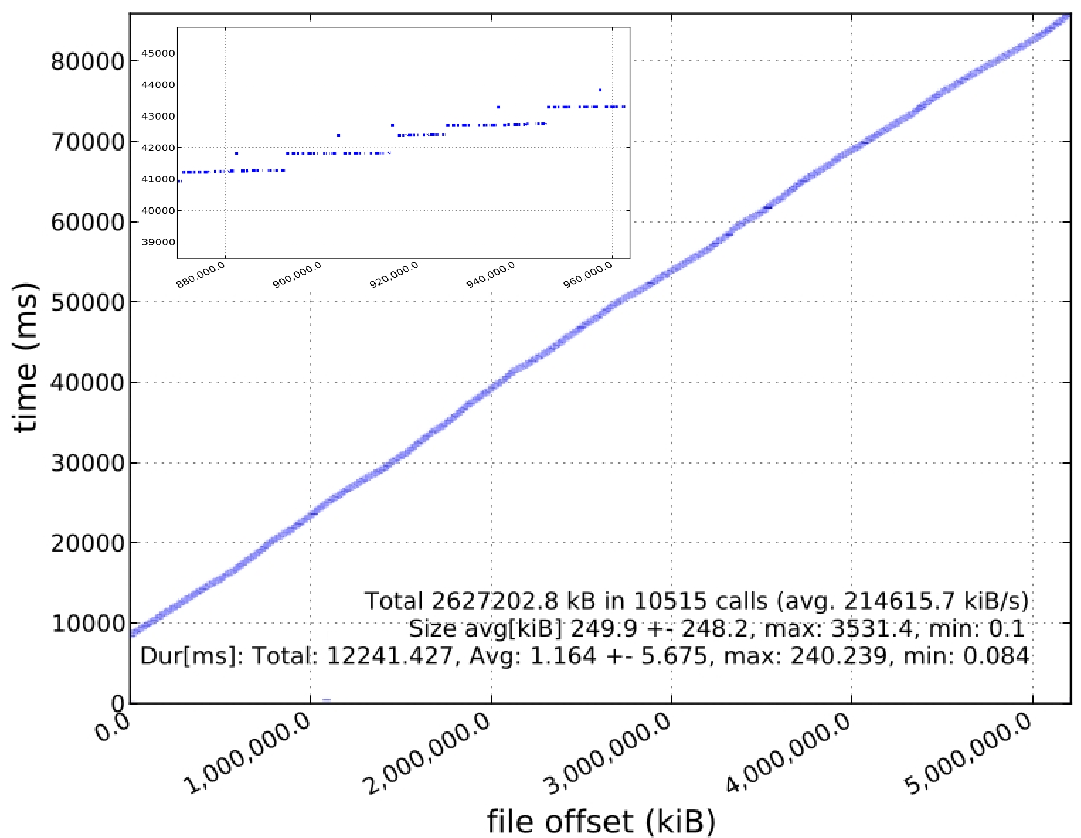
\includegraphics[width=0.35\textwidth]{figures/iopat_profile}
  \caption{I/O read profile of the target application under analysis extracted from the the GPFS file system in the test cluster.}
  \label{figure: iopattern_with_statistics}
\end{figure}
At a first glance the general I/O behaviour of the application looks linear, most of the accesses to the file follow an increasing offset. Nevertheless, adjacent reads are separated by gaps (strided read pattern). In a few cases this gap becomes negative, meaning that the application is moving backwards in the file to read some data previously left behind. After a detailed I/O pattern analysis we could divide the target file into contiguous non overlapping ranges. Within these ranges reads happen to have increasing offset. The information extracted was then used to tailor a configuration file containing the precise list of regions to prefetch. Additionally, we also used a configuration file containing only one prefetch region covering the whole file. This is intended to evaluate the relationship between costs and benefits when building a complex configuration file, instead of using a simple one that describes the general I/O behaviour of the application. 

Figure~\ref{figure: exec_time_comparison} and~\ref{figure: reads_final_comparison} show, respectively, the execution time and the number of completed reads for the target application in both clusters. 
\begin{figure}[!htb]
  \centering
  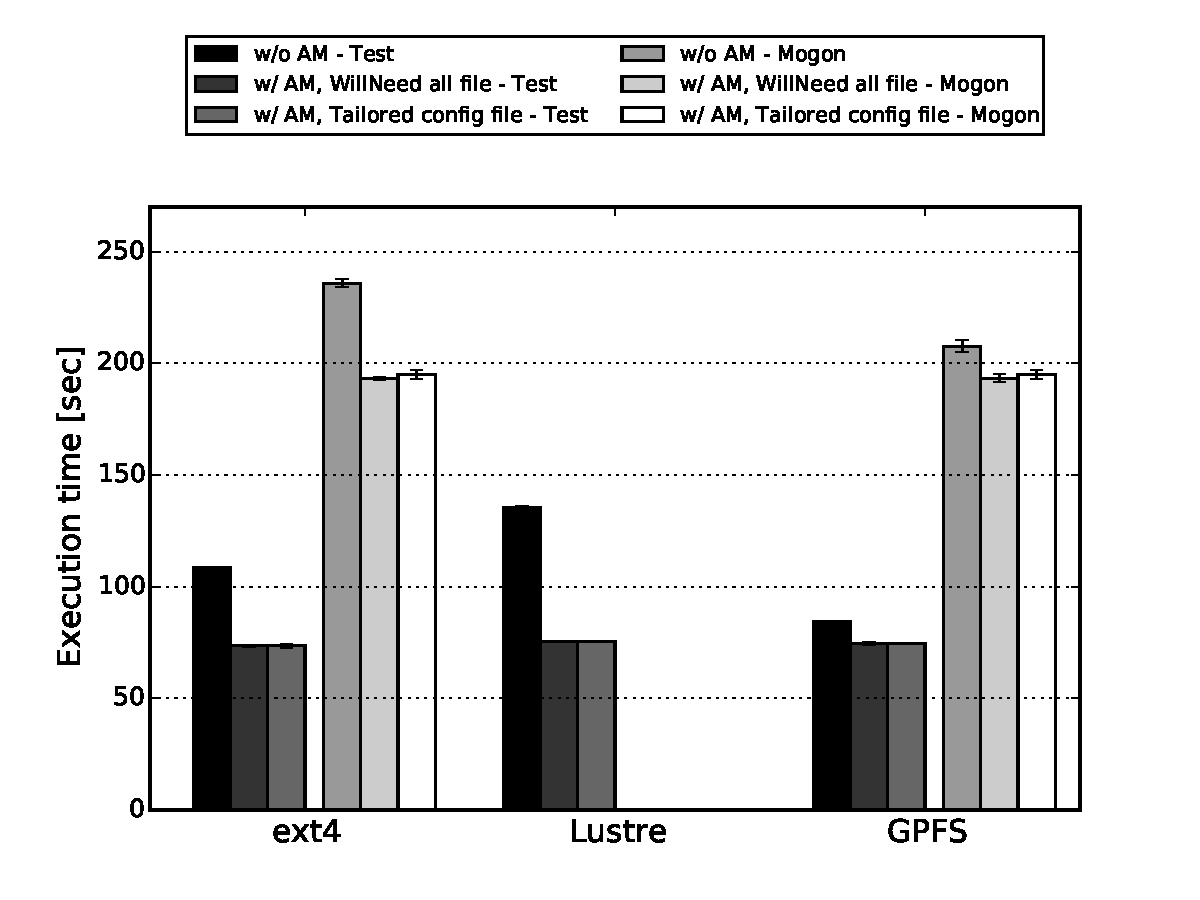
\includegraphics[width=0.4\textwidth]{figures/plot_runtime_inputfile_00050}
  \caption{Execution time of the target application on available file systems.}
  \label{figure: exec_time_comparison}
\end{figure}
\begin{figure}[!htb]
  \centering
  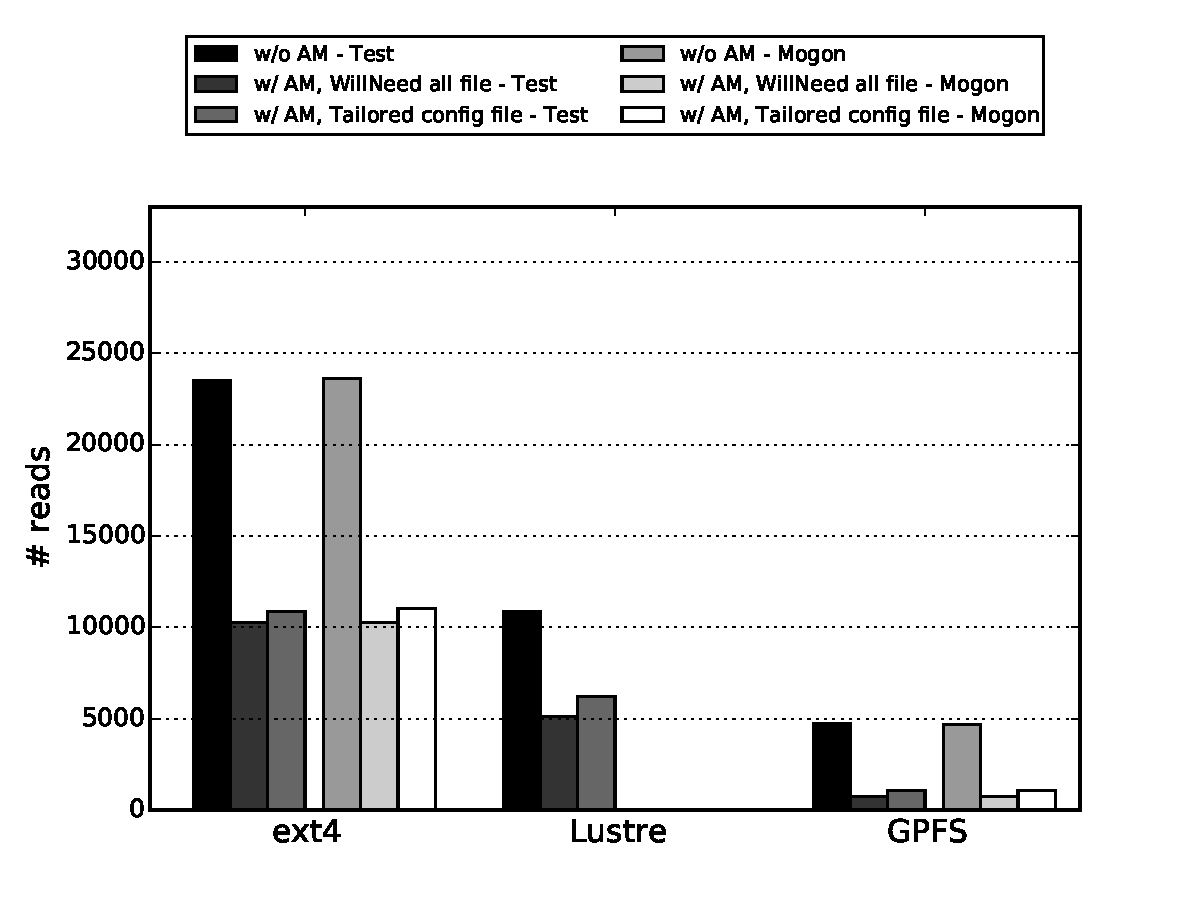
\includegraphics[width=0.4\textwidth]{figures/plot_reads_inputfile_00050}
  \caption{Number of read operations completed by the different file systems.}
  \label{figure: reads_final_comparison}
\end{figure}
The runtime shows an improvement of 11\% ($-10\ sec$) on Test Cluster and 6\% ($-13\ sec$) on Mogon for GPFS and 44\% ($-50\ sec$) on Test Cluster for Lustre. The number of reads is reduced by up to 83\% ($-3956$) on both Test Cluster and Mogon for GPFS and up to 52\% ($-5727$) on Test Cluster for Lustre. Similar improvements can be observed for ext4. 

From our analysis we can conclude that a configuration file describing the generic I/O behaviour of the application gives practically the same performance in terms of execution time as the tailored file containing precise information about what ranges shall (or shall not) be prefetched. This means that, specifically for the considered case, once we know the I/O behaviour of the application we can use one configuration file for every input, obtaining very good performance improvements with very little effort.

\section{Conclusions}
\label{sec: conclusions}
Before us, other works have used data prefetching to boost applications performance~\cite{HEBTAGGMCS13, ChangG99, ChenBSTG08, VanDeBogartFK09, TranR04, BynaCST08, ChenR10, HEST12}. Our approach differs from these works since we do not rely on precise I/O pattern information to predict and prefetch every chunck of data in advance. Instead we use data prefetching to group many small requests in a few big ones, improving applications performance and utilization of the whole storage system. Moreover, we provide the infrastructure that enables users to access file system specific interfaces for guided I/O without modifying applications and hiding the intrinsic complexity that such interfaces introduce.


\bibliographystyle{IEEEtran}
\bibliography{bibliography}


\end{document}

